The regular training procedure for a 4-feature model has a significant limitation. The model does not consider the feed-forward application of the prediction output.
In the case of excellent input values, the output is expected to be within 1 \% mis-accuracy since from 500 ideal SoC values, estimation of value 501 is a trivial task.

%
%
Two subplots, \mbox{Figure~\ref{fig:regular_tr}}, demonstrate the prediction results of a four-feature-based FUDS-trained simple LSTM model against a single battery cycle of DST driving.
\mbox{Figure~\ref{fig:regular_tr}a} demonstrates the prediction with input SoC based on "\textit{known}" perfect \textcolor{blue}{charge value} (i.e. from the training set) as subsequent prediction input at any random point in time, marked with a red dotted line (i.e. 500 values for SoC, with sensory data, from learning used to predict charge at 501).
On the other hand, the \mbox{Figure~\ref{fig:regular_tr}b} uses the feedforward approach, where only the first sample window has the true SoC (i.e. from the training set), and every upcoming prediction uses the calculated value from the previous step.
It therefore has a strict order of samples from start to end, marked as a yellow dotted line.
The same colour annotation will be used for all the remaining plots to distinguish the input schemes.
Clearly, the prediction very quickly diverges under normal Feed-Forward conditions as small predicted SoC inaccuracies rapidly accumulate. % and resemble the similarity with the Voltage curve during discharge.
This is a good justification for why there has been no evidence in the published literature of utilising a feed-forward approach for SoC estimation.
\ifthenelse{\boolean{thesis}}{
    \begin{figure}[htbp]
        \centering
        % DST based tests
        \begin{subfigure}[b]{0.485\textwidth}
            \centering
            % \includesvg[width=\linewidth]{III_Conclussion/im_compare/FUDS-val-48.svg}
            \includesvg[width=\linewidth]{III_Conclussion/im_compare/SMFUDS-val-9.svg}
            \caption{Regular training process snapshot}
            \label{subfig:regular_tr}
        \end{subfigure}
        \hfill
        \begin{subfigure}[b]{0.485\textwidth}
            \centering
            \includesvg[width=\linewidth]{III_Conclussion/im_compare/SMFUDS-FF-9.svg}
            \caption{Feed-Forward validation process snapshot}
            \label{subfig:regular_ts}
        \end{subfigure}
        \caption{Comparison between training and testing accuracies of a 4-featured based model with a default training and testing loop.}
        \label{fig:regular_tr}
    \end{figure}
} {
    \begin{figure*}[!t]
        \centering
        % \vspace{-3ex}
        % DST based tests
        \subfloat[Regular training process snapshot]{\includesvg[width=0.485\linewidth]{III_Conclussion/im_compare/SMFUDS-val-9-editted.svg}}
        \hfill
        \subfloat[Feed-Forward validation process snapshot]{\includesvg[width=0.485\linewidth]{III_Conclussion/im_compare/SMFUDS-FF-9.svg}}
        \caption{Comparison between training and testing accuracies of a 4-featured based \textcolor{blue}{LSTM} model with a default training and testing loop \textcolor{blue}{on the FUDS dataset}. Note that the error area fill has been removed from both plots due to an extremely large error in (b).}
        \label{fig:regular_tr}
    \end{figure*}
}
%
%
%
% The green error area axis has been dropped from \mbox{Figure~\ref{fig:regular_tr}b} due to high inaccuracy, which would cover half of the plot area.
% \ifthenelse{\boolean{thesis}}{The implementation of this prediction method is presented in \mbox{Appendix~\ref{app:Feed-Forward}}.}{}
% It demonstrates how the appended charge output model accumulates the error with every dependent input in a single prediction.
% If that output is used for further prediction and the model keeps preserving the dependency, the miss accuracy value rises non-linearly.

%
%
%! Get eid of that figgure, find a way to refer to it.
A key reason for the inaccuracies of the prediction in \mbox{Figure~\ref{fig:regular_tr}b} lies in the weights the model places on the \textcolor{blue}{SoC} input feature.
For a better weight balance, the training procedure must be modified to consider the possibility of an inaccuracy in the input charge data.
An example of a modified training loop can be found in the autoregressive models of \mbox{Lamberta et al.~\cite{time_2020}}, utilising methods of teacher forcing~\cite{brownlee_what_2017,orac_lstm_2024}.
The implementation can be applied to any early-created model, referring to regressive implementation.
% However, this is an example of the earlier mentioned stateful data management, where the model was explicitly programmed to run internally automatically and remains of stateless type.
% The state will be produced and used internally but is not present in the outputs.
% \ifthenelse{\boolean{thesis}}{\mbox{Figure~\ref{fig:autoregressive}} demonstrate how a trained model internally uses produced prediction to produce more than a single output ahead of time.
% For example, from a given input of sensory data of 23 days, a weather prediction model estimates a further three weeks ahead.
% However, this case produces the exact number of output features, matching the input to make the prediction work properly.
% Besides, once the 24 day comes, the same model can be updated with new actual information, adjusting the follow-up for three weeks.
% In the case of the State of Charge prediction model, such an approach cannot be used by itself since the SoC can not be determined like sensory data.
% \begin{figure}[ht]
%     \centering
%     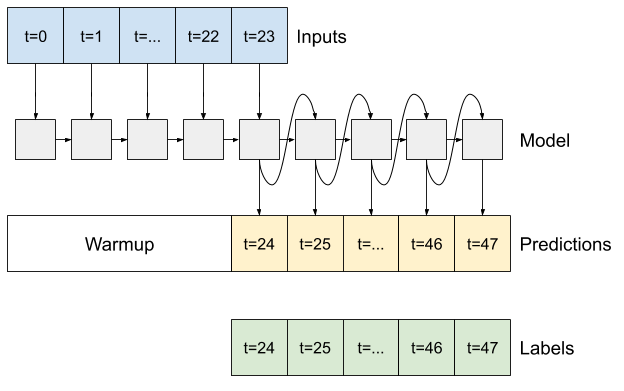
\includegraphics[width=\columnwidth]{II_Body/images/multistep_autoregressive.png}
%     \caption{Autoregressive model input and output demonstration from time-series tutorial~\cite{time_2020}}
%     \label{fig:autoregressive}
% \end{figure}
% } {
The implementation demonstration from time-series tutorial~\cite{time_2020} of the utilised Machine Learning framework provides both a written and visual explanation of autoregression implementation in the context of weather prediction ahead of time.
In the case of the \textcolor{blue}{SoC} prediction model, such an approach cannot be used by itself since the SoC can not be determined directly from sensory data (at least not during driving conditions).
Therefore, it will be adapted to overcome the problem of accumulated error in the feed-forward estimation method.
% }

%
%
\ifthenelse{\boolean{thesis}}{The SoC estimation model may benefit from multiple outputs by adapting the Autoregression to the accumulator utilisation scenario.
Therefore, the}
{The} training procedure for the regular LSTM model has been modified to consider potential inaccuracy in the known data rather than the future outputs.
The diagram in Figure~\ref{fig:training_testing} illustrates how the technique has been adapted to the current research.
\ifthenelse{\boolean{thesis}}{Unlike methods from the previous Chapter, the training and testing procedures were separated from each other.}
{Unlike the autoregressive example from the documentation tutorial~\cite{time_2020}, the training and testing procedures were separated from each other, and predictions happen not in the future, but over the already known data.}
% The diagram in \mbox{Figure~\ref{subfig:testing}} illustrates regular training and testing procedures for a model to produce output.
% The diagram in \mbox{Figure~\ref{fig:training_testing}a} demonstrates the procedure for the model call using autoregression during the training, whereas \mbox{Figure~\ref{fig:training_testing}b} only shows as a comparison to the regular usage and during the actual application or testing.
\ifthenelse{\boolean{thesis}}{Code-based detailed implementation have been attached in Appendix~\ref{app:AutoFeedback}.}{}

%
% ---->>>>>>>>>>.
% Unlike regular LSTM, training and testing differ from each other.
If the testing procedure remains unchanged, the training performs multiple calls during a single-window sample processing to actively incorporate its expected error.
For each window, rather than training all 500 samples in an instant, there is an iterative process between 490 and 500 if $AR_{width}$ is equal to 10, as an example.
While 490 samples of voltage, current, temperature and previous or known SoC values at time before $t$ will take a regular training process in the model and output the predicted SoC for $t+1$, every sample from $AR_{width}$ (10 in this case) will be processed in the model one by one with voltage, current and temperature, but along with every outputted SoC after 490th run at $t+r$.
\ifthenelse {\boolean{thesis}}{In this way, not only will the model output predicted SoC equal to $AR_{width}$ (Returned training array of 10 samples), but it also recursively trains on the inaccuracy that was produced by its last ten outputs, which the optimiser from Algorithm~\ref{alg:Adam} will attempt to minimise after passing through each window of 500 samples.}
{In this way, not only will the model output predicted SoC equal to $AR_{width}$ (Returned training array of 10 samples), but it also recursively trains on the inaccuracy that was produced by its last ten outputs, which the optimiser from Algorithm~\ref{alg:copyAdam} will attempt to minimise after passing through each window of 500 samples.}
The concept is similar to what RoAdam optimiser attempts to achieve to speed up the optimisation by directly incorporating the error in hyperparameters calculation.
Importantly, in real terms this greatly reduces the weighting put on input SoC in prediction, while still using those values to "ballpark" the location in the total SoC curve.

%
%
% In other words, every new call outputs the results and feeds again into the same model, with one sample from each sensor.
% Each output also contained a model state, containing the values stored in the NN' cells, preserving dependency between model calls for the Machine Learning framework utilisation only.
% Intentinally, with time, it will get minimised.
% State output is used only for internal model processing.
% Every output of every step has been stored in the returned array for the optimiser to adjust weights.
With a new approach, the optimiser will compare an array of predicted samples against the actual values of the SoC, making adjustments based on the inaccuracies present in the dependencies and considering them as part of the system, to update weights accordingly.
Unlike testing, the training is not feed-forward based; therefore, all actual SoC data and known SoC inputs are considered true, except the last $AR_{width}$, which matches the number of outputs and is used only by the optimiser, not at training, therefore being excluded from input arrays $t_{n+...}$ on Figure~\ref{fig:training_testing}.
To compare this process with the standard approach, using predicted SoC in the feed-forward manner will assume that the history 500 samples have been perfectly correct, leading to error accumulation and divergence from the actual value.
% This was meant to increase the model fit process.
The more output samples the model returns during the training (returned training array), the longer the training process becomes, but the better the real-time prediction against aggressive driving profiles gets.
For training, that process is done purely for one window, which means, they still can be shuffled in any order, if necessary.
That regressive process of using only the last several samples with some error produced by the models' prediction is far more efficient than adding a random noise level in the array of known SoC and adjusting to what level brings better results for each driving profile.
% By minimising the error from AR-width number of predicted SoC using the optimiser, the imperfection of the SoC in the history becomes included to the models' weights.
\ifthenelse{\boolean{thesis}}{
    \begin{figure}[htbp]
        \centering
        % DST based tests
        \begin{subfigure}[b]{0.85\textwidth}
            \centering
            % 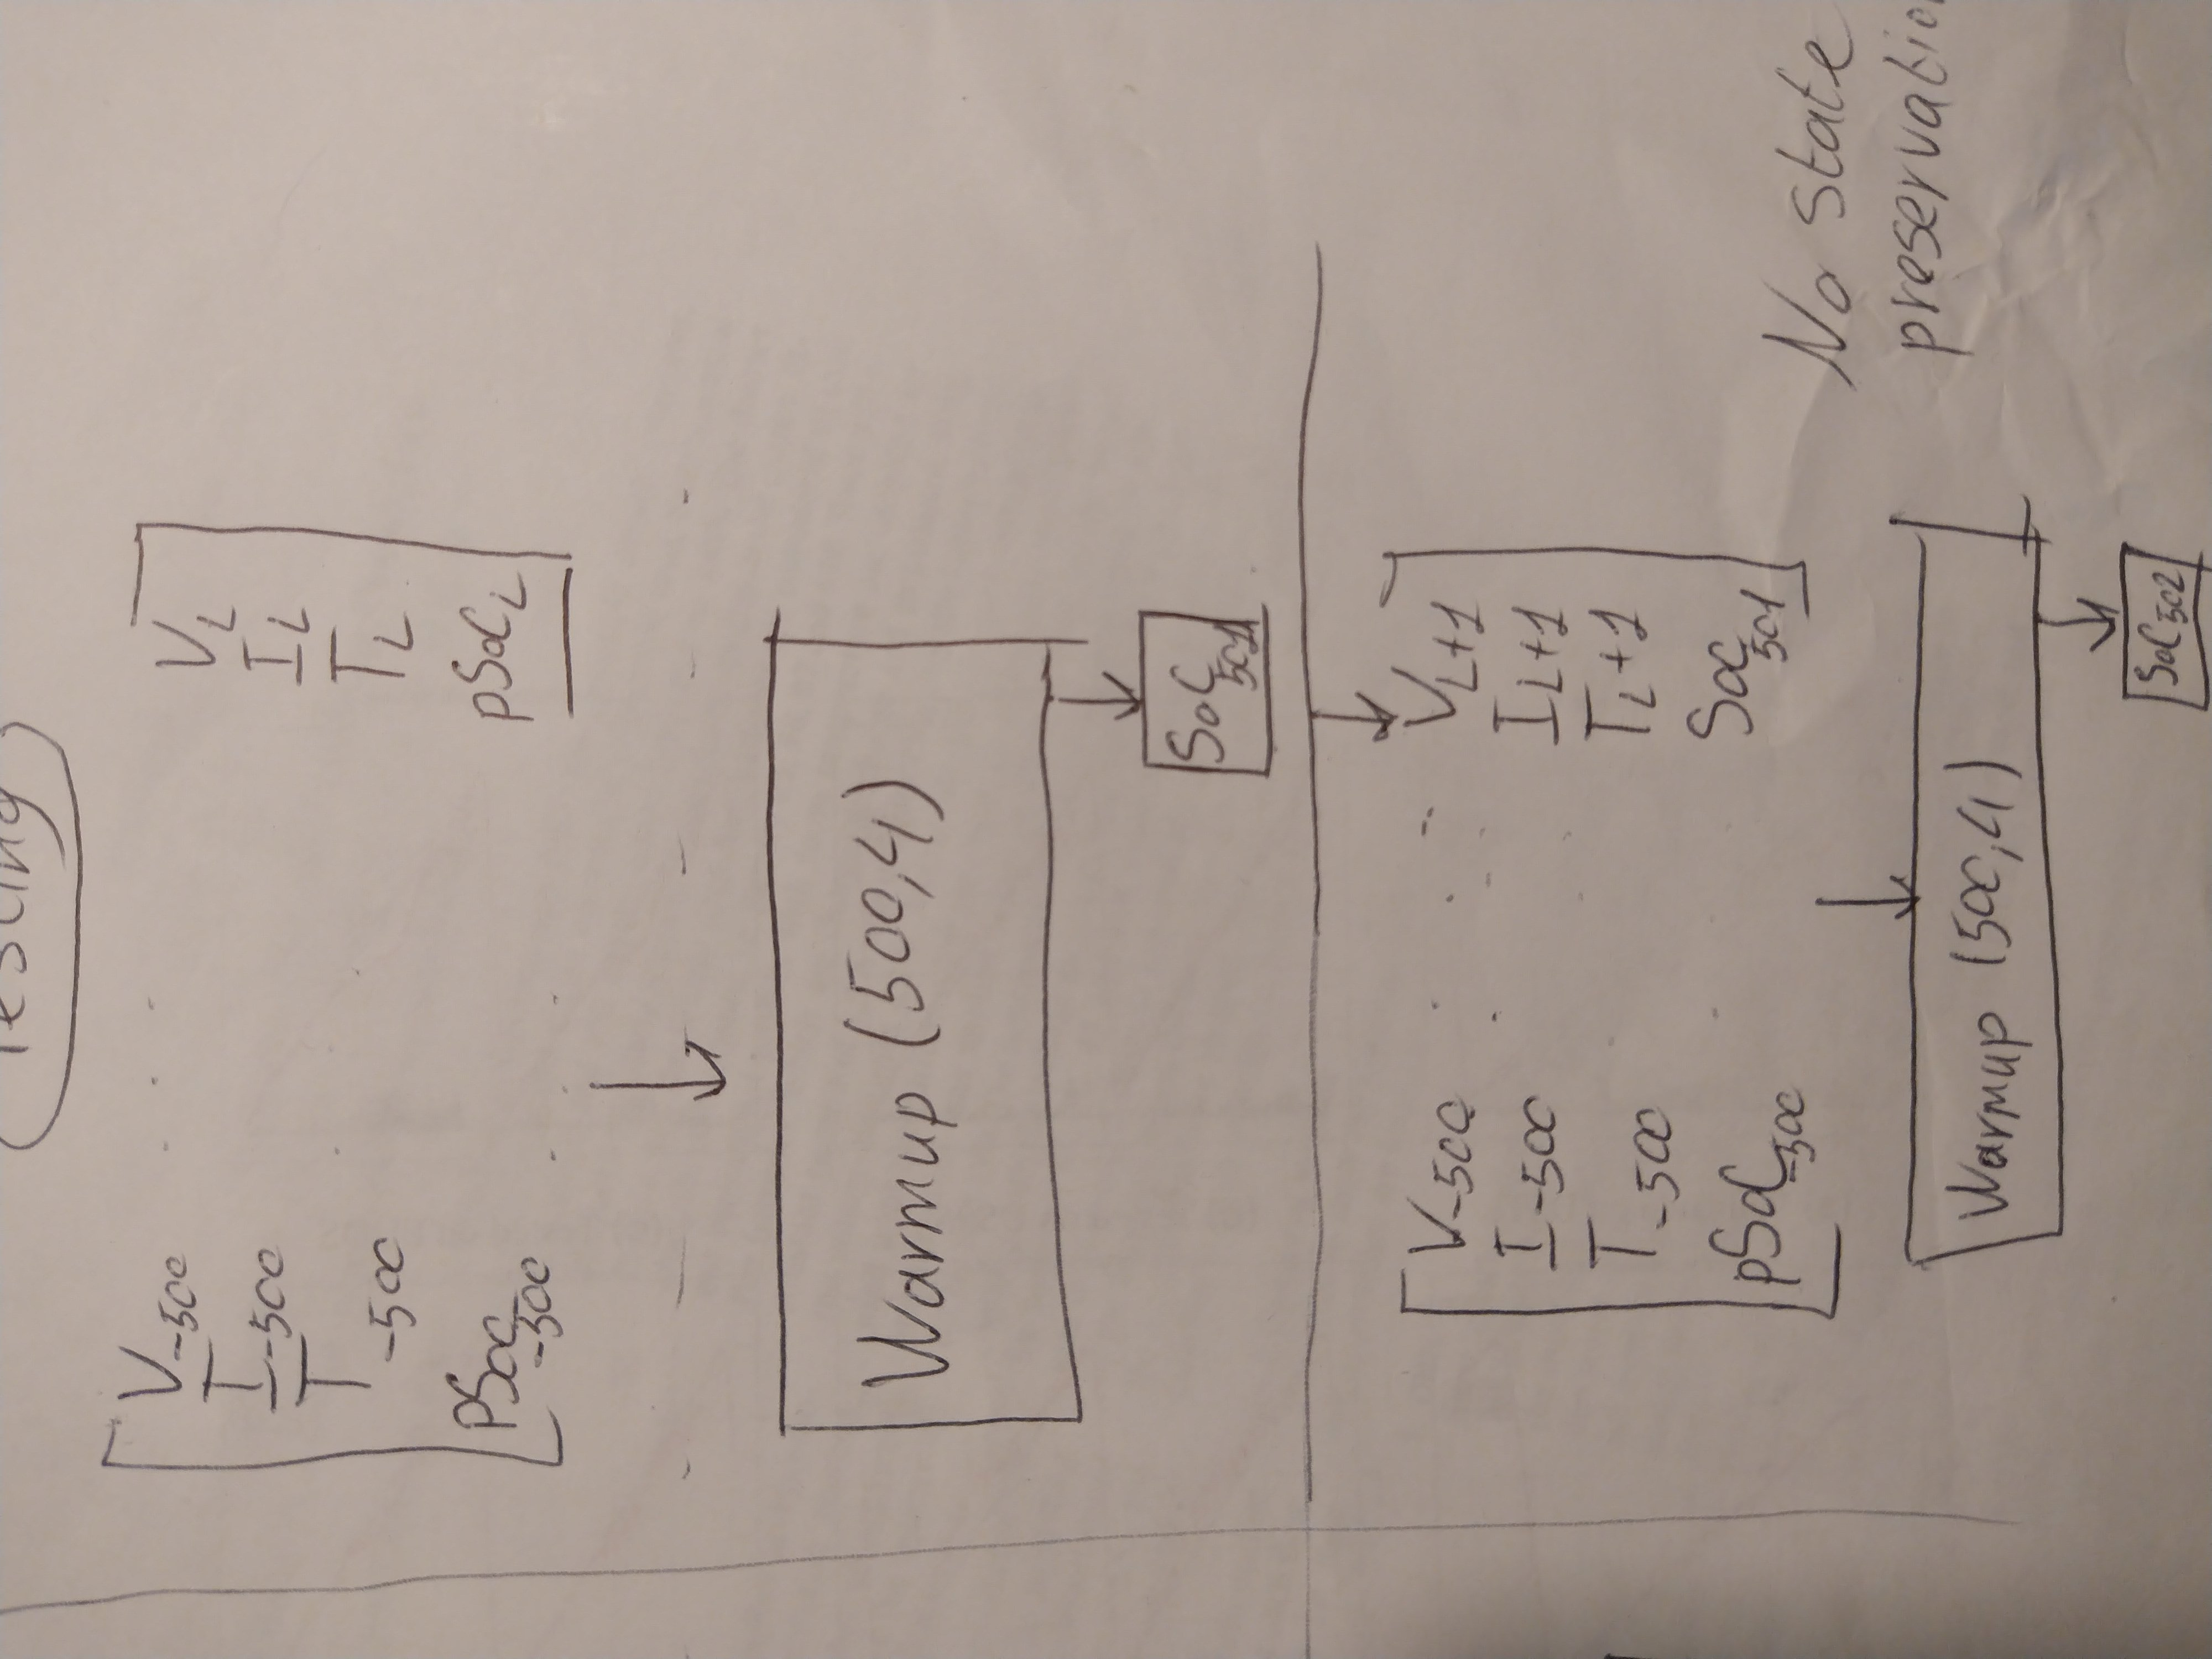
\includegraphics[width=\linewidth]{II_Body/images/IMG_20210524_133103.jpg}
            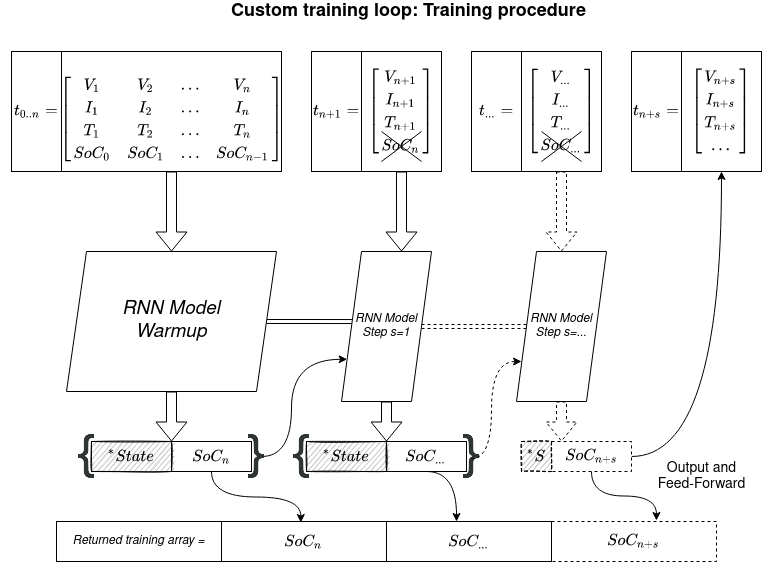
\includegraphics[width=\linewidth]{II_Body/images/Autoregression-Training.png}
            \caption{Custom autoregressive training procedure}
            \label{subfig:training}
        \end{subfigure}
        \hfill
        \begin{subfigure}[b]{0.85\textwidth}
            \centering
            % 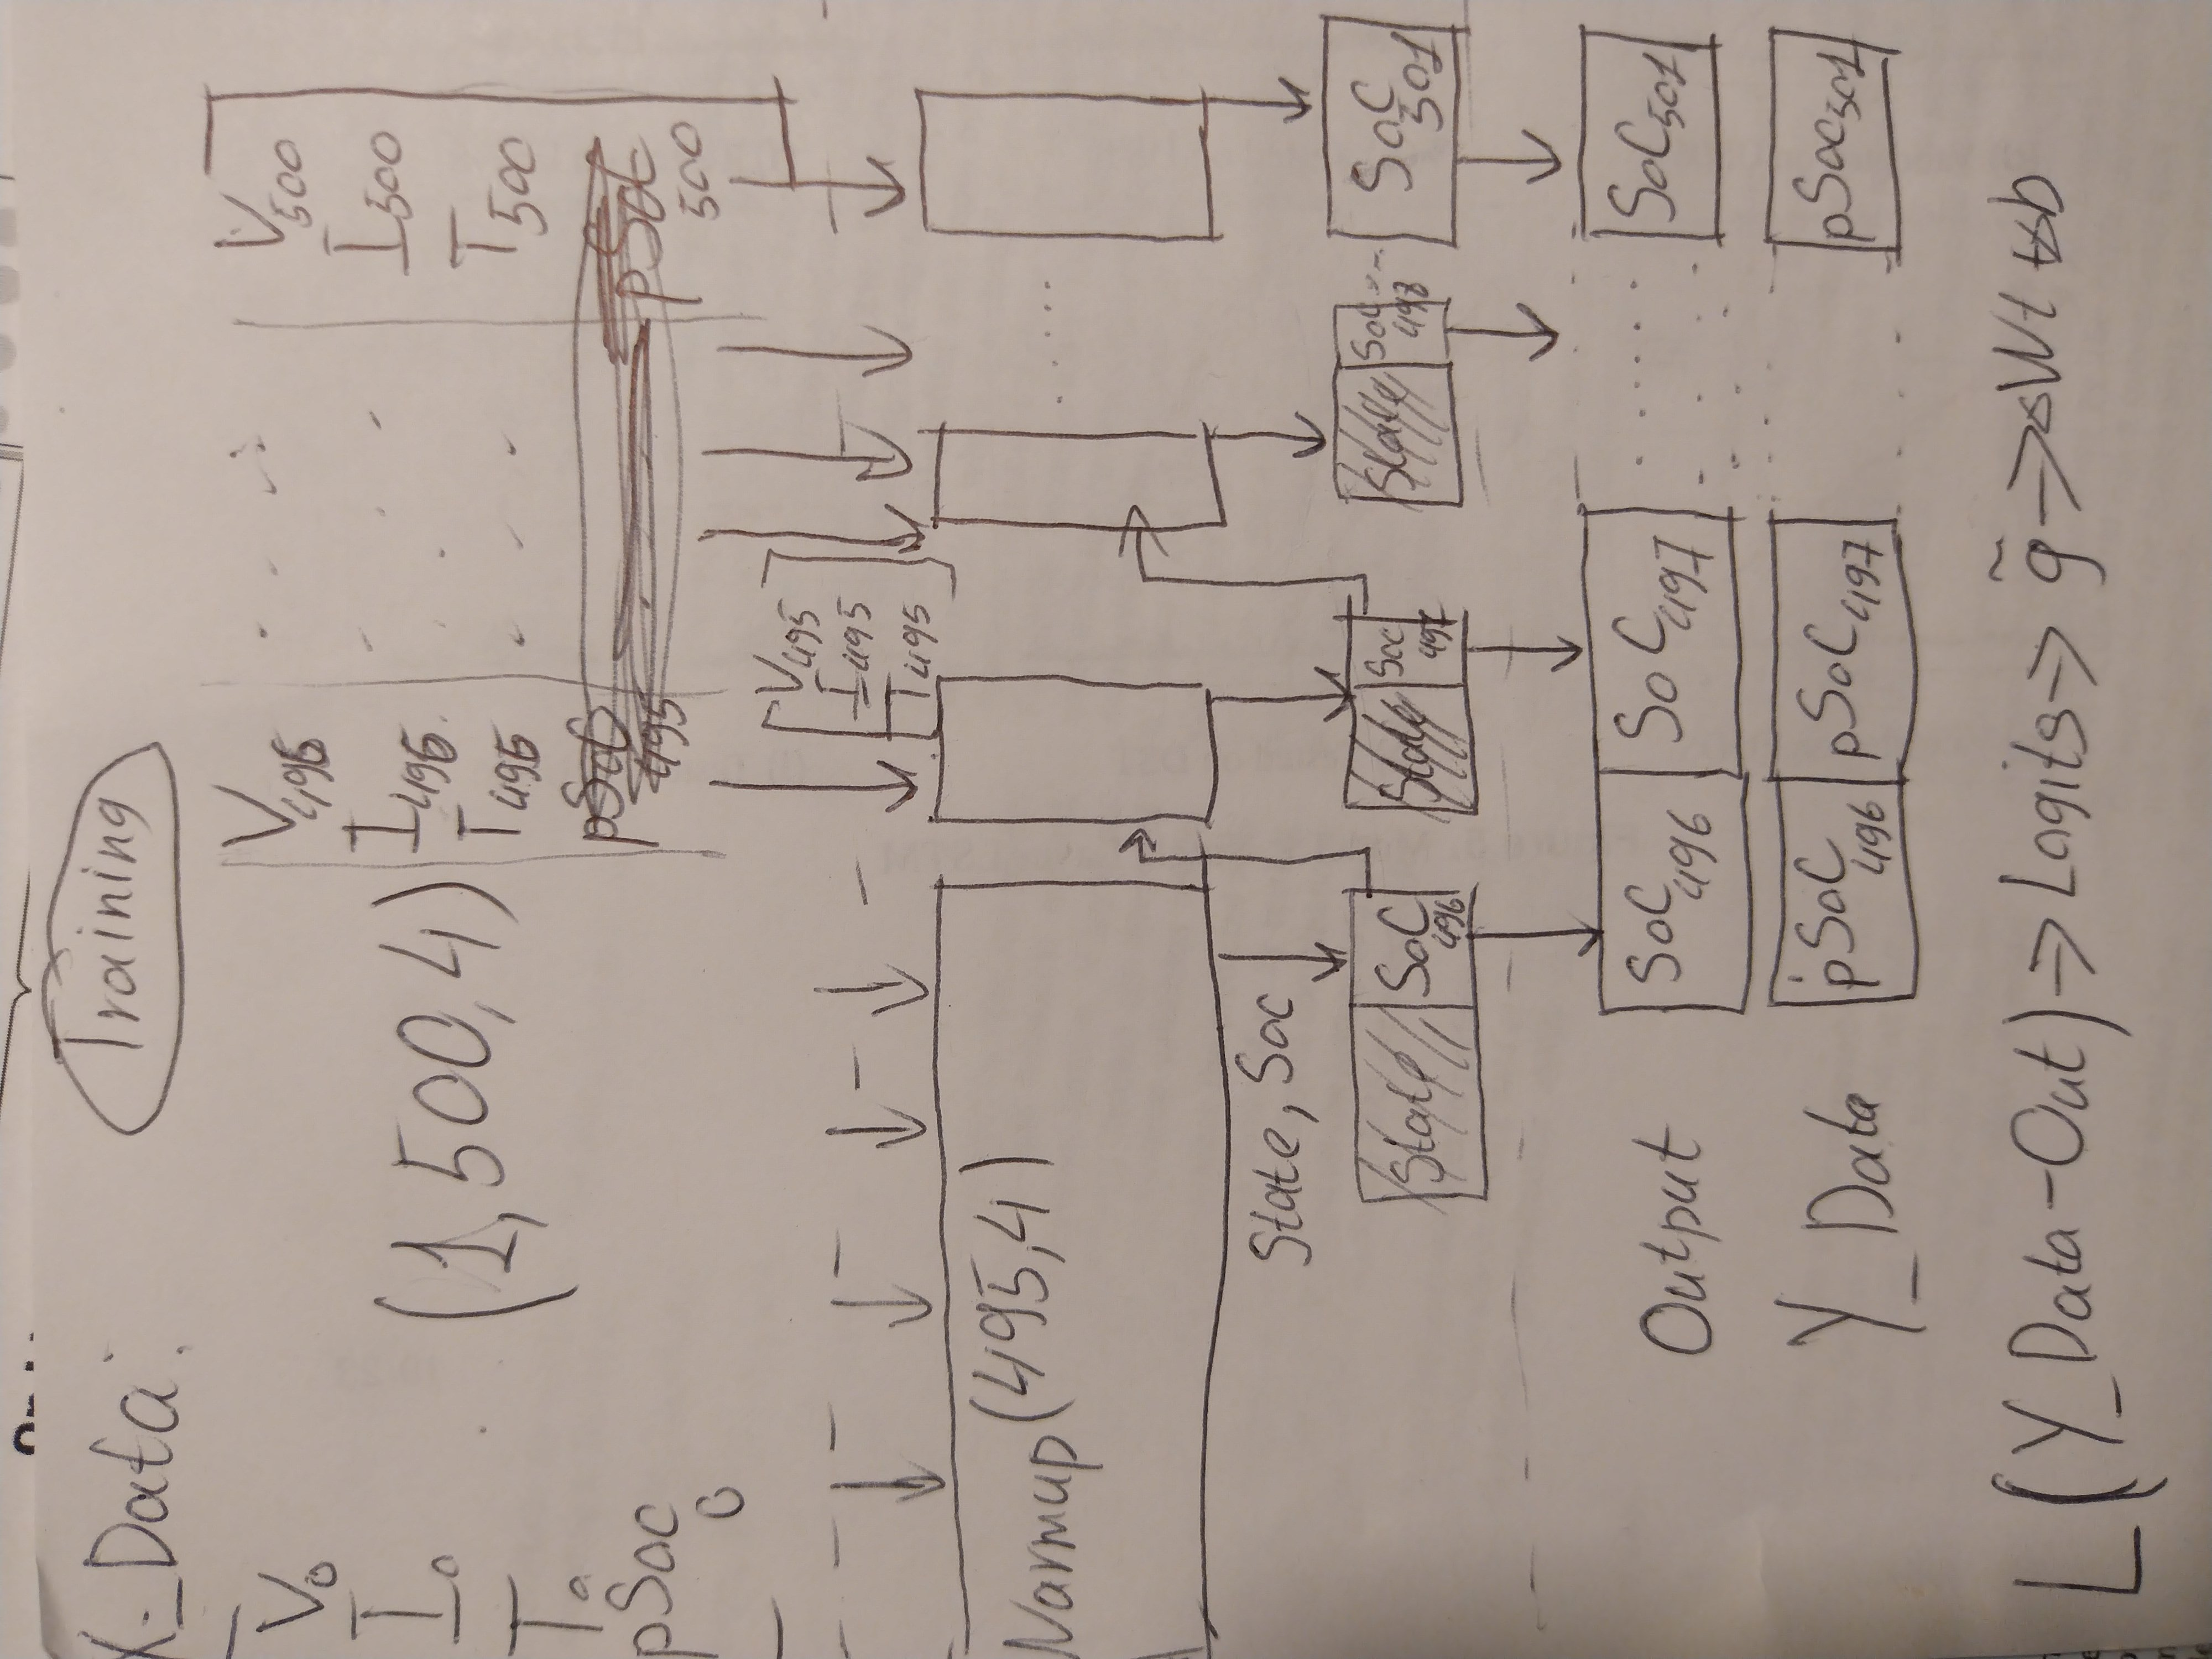
\includegraphics[width=\linewidth]{II_Body/images/IMG_20210524_133052.jpg}
            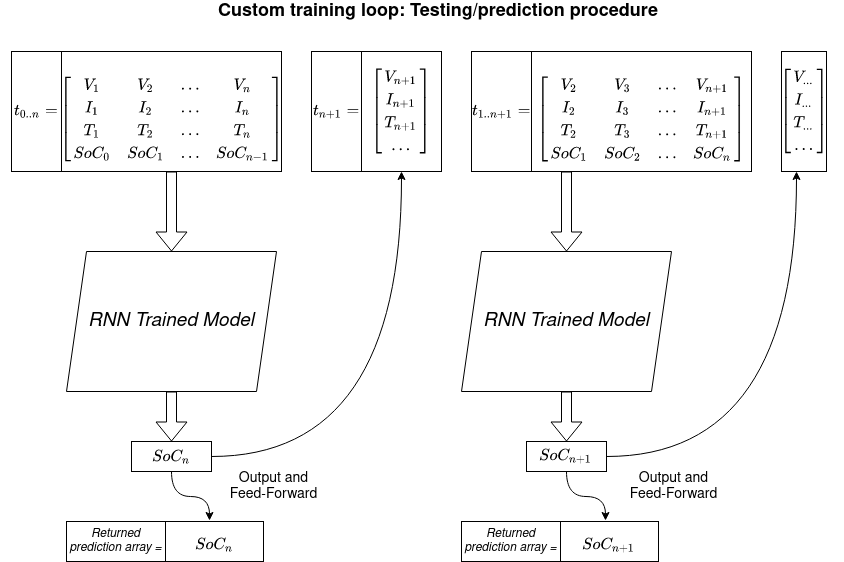
\includegraphics[width=\linewidth]{II_Body/images/Autoregression-Testing.png}
            \caption{Regular testing and validation procedure}
            \label{subfig:testing}
        \end{subfigure}
        \caption{Block diagram demonstration of training and testing working procedures for 4-featured-based models.}
        \label{fig:training_testing}
    \end{figure}
} {
    % \begin{figure*}[!t]
    %     \centering
    %     % DST based tests
    %     \subfloat[Custom autoregressive training procedure]{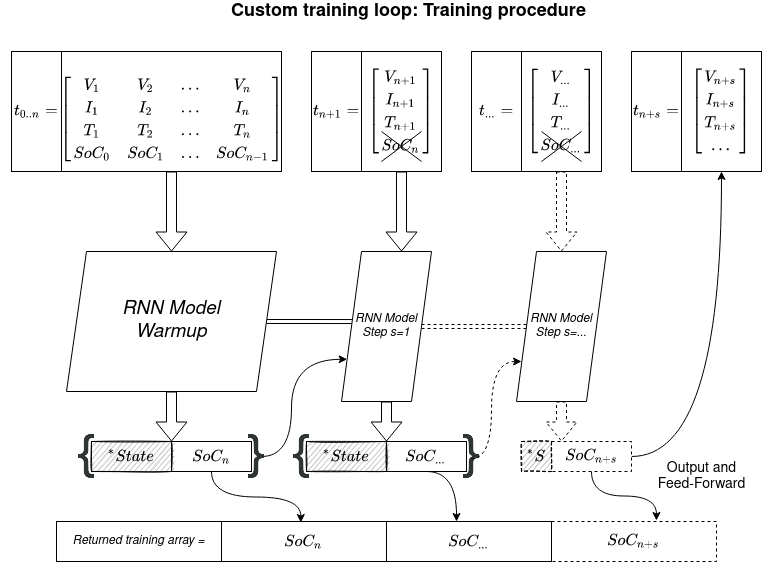
\includegraphics[width=0.85\linewidth]{II_Body/images/Autoregression-Training.png}}
    %     \hfill
    %     \subfloat[Regular testing and validation procedure]{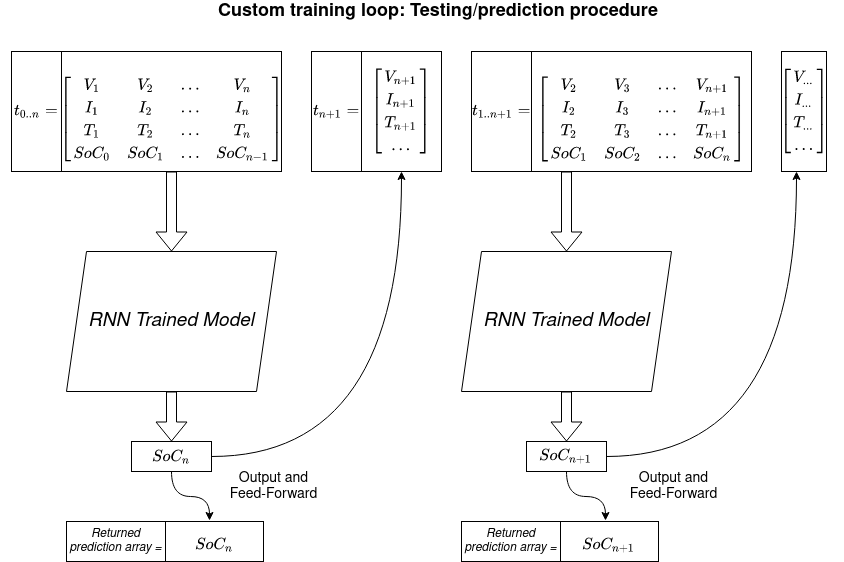
\includegraphics[width=0.85\linewidth]{II_Body/images/Autoregression-Testing.png}}
    %     \caption{Block diagram demonstration of training and testing working procedures for 4-featured-based models.}
    %     \label{fig:training_testing}
    % \end{figure*}
    \begin{figure*}[!t]
        \centering
        % DST based tests
        \includesvg[width=\linewidth]{II_Body/images/Autoregression_updated-Training.svg}
        \caption{Block diagram demonstration of custom autoregressive training procedure for 4-featured-based models, where $n$ is the initial number of input samples, excluding the $AR_{width}$ $(r)$. The sum of $n$ and $r$ is equal to 500 samples for this research.}
        \label{fig:training_testing}
    \end{figure*}
}

%
%
Now, with modified training procedure and optimiser incorporating 30 samples of $AR_{width}$, as an example, \mbox{Figure~\ref{fig:modefied_tr}} contains a similar test, as without autoregression on earlier Figure~\ref{fig:regular_tr}.
Even though the accuracy with tabled samples has decreased between \mbox{Figure~\ref{fig:regular_tr}a and~\ref{fig:modefied_tr}a}, its feed-forward prediction accuracy has significantly increased and does not lose the trend.
The implementation has been based on contributions from the original framework developers~\cite{time_2020} and written based on corresponding original documentation of Tensorflow 2.4~\cite{tensorflow2015-whitepaper}.
\ifthenelse{\boolean{thesis}}{
\begin{figure}[H]
    \centering
    \begin{subfigure}[b]{0.485\textwidth}
        \centering
        % \includesvg[width=\linewidth]{III_Conclussion/Models/Sadykov2021-30steps/FUDS-models/SMRFUDSval-19.svg}
        \includesvg[width=\linewidth]{III_Conclussion/im_compare/SMRFUDSval-19.svg}
        \caption{Modified training process}
        \label{subfig:modefied_tr}
    \end{subfigure}
    \begin{subfigure}[b]{0.485\textwidth}
        \centering
        % \includesvg[width=\linewidth]{III_Conclussion/Models/Sadykov2021-30steps/FUDS-models/SMRFUDS-FF-19.svg}
        \includesvg[width=\linewidth]{III_Conclussion/im_compare/SMRFUDS-FF-19.svg}
        \caption{Feed-Forward validation process}
        \label{subfig:modefied_ts}
    \end{subfigure}
    \caption{Comparison between training and testing accuracies of a 4-featured based model with a modified training and default testing loops.}
    \label{fig:modefied_tr}
\end{figure}
} {
\begin{figure*}[!t]
    \centering
    \vspace{-3ex}
    \subfloat[Modified training process]{\includesvg[width=0.485\linewidth]{III_Conclussion/im_compare/SMRFUDSval-19.svg}}
    \label{subfig:modefied_tr}
    \subfloat[Feed-Forward validation process]{\includesvg[width=0.485\linewidth]{III_Conclussion/im_compare/SMRFUDS-FF-19.svg}}
    \label{subfig:modefied_ts}
    \caption{Comparison between training and testing accuracies of a 4-featured based LSTM model with a modified training and default testing loops, \textcolor{blue}{and $AR_{width}$ of 30 steps}.}
    \label{fig:modefied_tr}
\end{figure*}
}
